\documentclass[12pt,a4paper,ngerman]{article}
\usepackage{babel}
%\usepackage{natbib}
\usepackage{url}
%\usepackage[left=2cm, right=1.5cm, top=2cm, bottom=2cm]{geometry}
%\usepackage[ansinew]{inputenc}
\usepackage{amsmath}
\usepackage{nicefrac} % macht schöne Brüche mit querstrich mit \nicefrac{1}{2}
\usepackage{graphicx}
%\graphicspath{}
\usepackage{titlesec}% um chapterüberschriften anzupassen.
\titleformat{\chapter}{\normalfont\huge\bf}{\thechapter.}{20pt}{\huge\bf}
\usepackage{parskip}
\usepackage{fancyhdr}
\usepackage{amsfonts}
\usepackage{float}
\usepackage{caption}
\usepackage{subcaption} % for \begin{subfigure}
	
\usepackage{csquotes} % mit \enquote{blabla} tolle anfürungsstriche erstellen
%\usepackage{physics} %lässt mich \bra und \ket benuzen %im konflict mit siunitx
\usepackage{amssymb} % für \gtrsim und \lesssim

\usepackage{pgfplots} %für plots
\pgfplotsset{compat=newest}

\usepackage{varioref} % macht mit \vref{} viel bessere referenzen
\usepackage{hyperref} % macht klickbare referenzen

\usepackage{xcolor, soul} %mit \hl{} kann man toll Sachen hervorheben.
\newcommand{\highlight}[1]{%
	\colorbox{yellow!50}{$\displaystyle#1$}} % mit \highlight{} kann man sogar in Gleichungen hervorheben

\usepackage{vmargin}
\usepackage[section]{placeins}
\usepackage{capt-of}
\usepackage{enumitem}
\usepackage{multirow}
\usepackage{blindtext}
\usepackage{lipsum}
\usepackage[version=4]{mhchem} % um Chemische Elementsymbole zu benutzen: \ce{H20}

\usepackage{pdfpages} % um PDFs einzufügen

%spread to latex:
\usepackage{booktabs, multirow} % for borders and merged ranges
\usepackage{changepage,threeparttable} % for wide tables

\providecommand{\e}[1]{\ensuremath{\cdot 10^{#1}}}
\providecommand{\fehlt}{\textcolor{red}{{ ¡Fehlt! }}}
\providecommand{\mytitle}{Plasmakristalle}

\usepackage{siunitx}
\sisetup{
	separate-uncertainty = true,
	%per-mode = fraction,
	%per-mode = symbol
}
\DeclareSIUnit\bar{bar}
\DeclareSIUnit\px{px}
\DeclareSIUnit\atomicmassunit{u}
\DeclareSIUnit\elemtLad{e}
\usepackage{isotope}


\setmarginsrb{3 cm}{2.5 cm}{3 cm}{2.5 cm}{1 cm}{1.5 cm}{1 cm}{1.5 cm}
\title{\mytitle} % Title


\author{Frederik Uhlemann, Florian Adamczyk}
% Author
\date{\today}
% Date

\makeatletter
\let\thetitle\@title
\let\theauthor\@author
\let\thedate\@date
\makeatother

\pagestyle{fancy}
\fancyhf{}
\rhead{\theauthor}
\lhead{\mytitle}
\cfoot{\thepage}
%%%%%%%%%%%%%%%%%%%%%%%%%%%%%%%%%%%%%%%%%%%%
\begin{document}
		
	%%%%%%%%%%%%%%%%%%%%%%%%%%%%%%%%%%%%%%%%%%%%%%%%%%%%%%%%%%%%%%%%%%%%%%%%%%%%%%%%%%%%%%%%%
	
	\begin{titlepage}
		\centering
		\vspace*{0.5 cm}
		% \begin{large} Justus-Liebig-Universität\\ Gießen \end{large}
		\frame{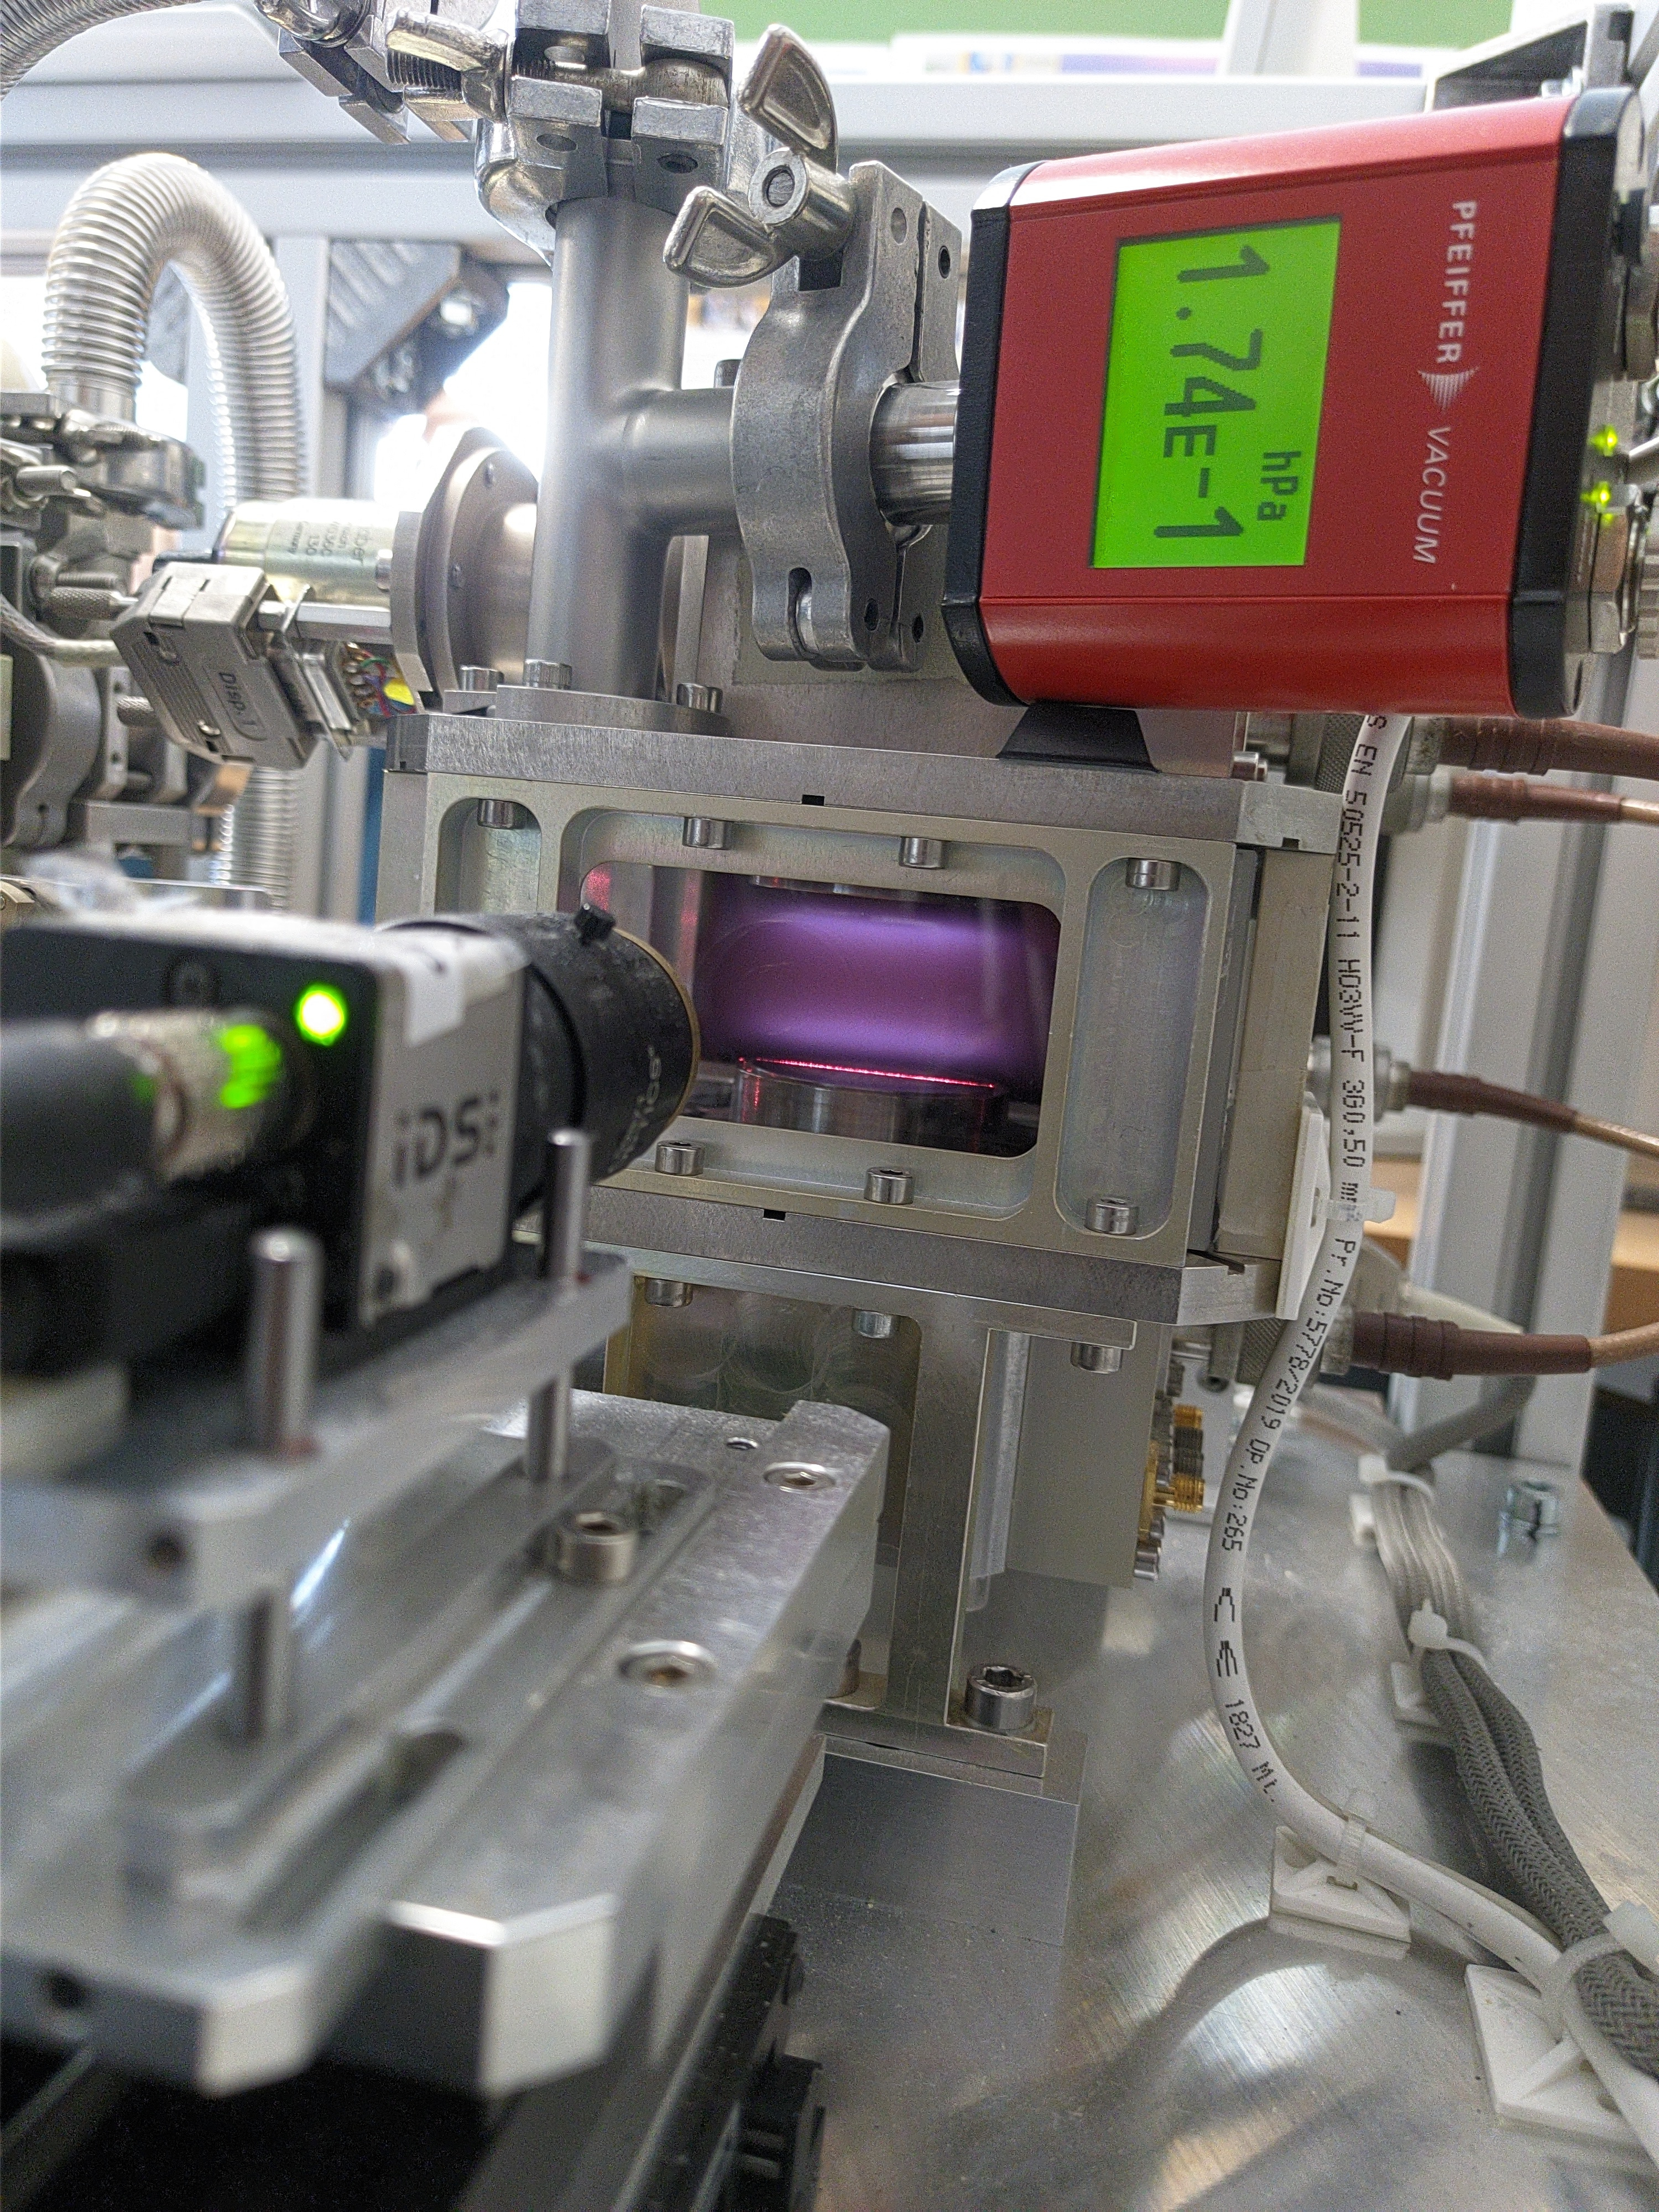
\includegraphics[width = 0.5 \textwidth]{fotos/foto3.jpg}}
		\\[.5 cm]
		% \begin{center}    \textsc{\Large Justus - Liebig - Universität}\\{Giessen}\\[0.8cm]	\end{center}% University Name
		Versuch 7 des\\
		\textsc{\Large Fortgeschrittenen-Praktikums}\\ [0.3 cm]				% Course Code
		\rule{\linewidth}{0.2 mm} \\[0.4 cm]
		{ \huge \bfseries \thetitle}\\
		\rule{\linewidth}{0.2 mm}\\
		Versuchstermin 22.07.2024 \\
		~ \\
		[.5 cm]
		
		
		\begin{minipage}{0.49\textwidth}
			\begin{flushleft}
				 \emph{Praktikumsbetreuer:}\\
				 Michael Kretschmer\\
				 %  Affiliation\\
				 \small{\href{mailto:michael.kretschmer@exp1.physik.uni-giessen.de}{michael.kretschmer@exp1.physik.uni-giessen.de}}
			\end{flushleft}
		\end{minipage}~
		\begin{minipage}{0.49\textwidth}
			\begin{flushright}
				\emph{Protokoll von:} \\
				
				\large{Frederik Uhlemann}\\
				\small{\href{mailto:frederik-vincent.uhlemann@physik.uni-giessen.de}{frederik-vincent.uhlemann@physik.uni-giessen.de}\\~\\
					%Matrikel Nr.: \:  \\[0.5cm]
					%\href{mailto:}{}
				}
				\large{Florian Adamczyk} \\
				\small{\href{mailto:florian.marius.adamczyk@physik.uni-giessen.de}{florian.marius.adamczyk@physik.uni-giessen.de}\\
					%Matrikel Nr.: \: 8105234}
			}
		\end{flushright}
	\end{minipage}
	
	\end{titlepage}
	
%%%%%%%%%%%%%%%%%%%%%%%%%%%%%%%%%%%%%%%%%%%%%%%%%%%%%%%%%%%%%%%%%%%%%%%%%%%%%%%%%%%%%%%%%
\setcounter{secnumdepth}{3}
\setcounter{tocdepth}{3}
% \tableofcontents
%\newpage

%%%%%%%%%%%%%%%%%%%%%%%%%%%%%%%%%%%%%%%%%%%%%%%%%%%%%%%%%%%%%%%%%%%%%%%%%%%%%%%%%%%%%%%%%
%\renewcommand{\thesection}{\arabic{section}} %lässt in den subsections die erste zahl von darüberliegenden chapter weg.

%\pagebreak
	
%\setcounter{chapter}{-1}
\section*{Zielsetzung}\addcontentsline{toc}{chapter}{Einleitung}
Im Rahmen des Versuchs \glqq{}Plasmakristall\grqq{} wird die Erzeugung und Untersuchung eines Plasmakristalls in einer Niederdruckkammer angestrebt. Hierbei wird ein Plasma aus Argon-Gas erzeugt, in das Mikropartikel aus Plastik eingebracht werden. Diese Partikel laden sich negativ auf und ordnen sich unter geeigneten Bedingungen zu einem Kristall. Ziel des Experiments ist es, die Kristallstruktur, die Abstände zwischen den Partikeln sowie den Übergang zur flüssigen Phase zu analysieren. Die Beobachtung und Analyse der Kristallbildung erfolgt mithilfe eines Lasers und einer Digitalkamera, die es ermöglichen, die Strukturen ebenenweise zu erfassen und zu dokumentieren. Die gewonnenen Daten werden anschließend mit theoretischen Modellen und den Eigenschaften idealer Kristalle verglichen, um ein tieferes Verständnis der physikalischen Prozesse zu erlangen.

	% notiz an mich: mit "~ bewirke ich einen geschützten bindestrich an dem nicht getrennt werden darf.
	% nur eine ~ macht ein geschütztes (normales) Leerzeichen. \, macht ein halbes geschütztes Leerzeichen.

\section{Theorie}
\subsection{Einleitung} Der Begriff \glqq{}Plasmakristall\grqq{} mag auf den ersten Blick widersprüchlich erscheinen, da man in der Plasmaphase keine geordneten Strukturen erwartet. Normalerweise ist es erforderlich, dass ein System von der gasförmigen über die flüssige in die feste Phase übergeht, um kristalline Strukturen zu bilden. In einem herkömmlichen Plasma ist dies nicht möglich. Allerdings können in komplexen, mehrkomponentigen Plasmen unter bestimmten Bedingungen geordnete Strukturen auftreten. Ein Beispiel hierfür sind Mikropartikel aus Plastik, die sich in einem Niedertemperaturplasma zu einer kristallartigen Anordnung formieren können, was als Plasmakristall bezeichnet wird.

\paragraph{Die theoretische Vorhersage} des Plasmakristalls erfolgte 1986, und der experimentelle Nachweis gelang 1994 am Deutschen Zentrum für Luft- und Raumfahrt (DLR) in Köln in Zusammenarbeit mit dem Max-Planck-Institut für extraterrestrische Physik (MPE) in Garching. Die Untersuchung von Plasmakristallen ist ein aktuelles Forschungsgebiet, das sowohl für die Grundlagenforschung als auch für Anwendungen in der Materialwissenschaft und der Astrophysik von Interesse ist.

\section{Plasma als vierter Aggregatzustand}
Plasma wird oft als der vierte Aggregatzustand bezeichnet, bei dem die Atome ionisiert vorliegen. Dies bedeutet, dass die Elektronen von den Atomkernen getrennt und somit frei beweglich sind. Plasmen werden je nach den Eigenschaften ihrer Teilchen in verschiedene Kategorien eingeteilt:

\begin{itemize}
    \item \textbf{Relativistisches Plasma:} Liegt vor, wenn die kinetische Energie der Elektronen etwa 30 \% der Lichtgeschwindigkeit beträgt.
    \item \textbf{Quantenmechanisches Plasma:} Hierbei ist die de-Broglie-Wellenlänge der Plasmateilchen größer als der Abstand zwischen den Teilchen.
    \item \textbf{Ideales Plasma:} Die Coulomb-Wechselwirkungsenergie zwischen den Teilchen ist schwächer als die thermische Energie der Teilchen.
    \item \textbf{Niedertemperaturplasma:} Der Ionisationsgrad \( \frac{n_i}{n_i + n_g} \ll 1 \), wobei \( n_i \) die Dichte der ionisierten und \( n_g \) die Dichte der neutralen Gasatome ist.
\end{itemize}

In diesem Experiment wird ein nicht-relativistisches, klassisches, stark gekoppeltes Niedertemperaturplasma verwendet.

\subsection{Plasmakristall}
In einem normalen Plasma sind die Teilchen frei beweglich, was eine Kristallstruktur verhindert. Ein sogenanntes komplexes Plasma, dem kleine, feste Kügelchen (Durchmesser etwa 1 µm) hinzugefügt werden, ermöglicht jedoch die Bildung eines Plasmakristalls. Diese Partikel laden sich durch Stöße mit den freien Elektronen auf und interagieren über Coulomb-Wechselwirkungen. Unter geeigneten Bedingungen entsteht eine geordnete Struktur, die als Plasmakristall bezeichnet wird. Ein elektrisches Feld hält den Kristall in Schwebe, und er kann mithilfe eines Lasers beobachtet werden. Reibungskräfte und Thermophorese, die Bewegung der Teilchen entlang eines Temperaturgradienten, beeinflussen zusätzlich die Kristallstruktur.

\subsection{Struktur des Kristalls}
Ein Kristall zeichnet sich durch Fernordnung aus, was bedeutet, dass die Abstände der Atome oder Partikel periodisch sind. Die Paarkorrelationsfunktion \( g(r) \) ist ein Maß für die Wahrscheinlichkeit der Fernordnung. Sie gibt den Erwartungswert an, dass sich im Abstand \( r \) von einem Teilchen \( i \) ein anderes Teilchen \( j \) befindet. Bei Vorliegen von Fernordnung zeigt die Funktion \( g \) gegen \( r \) periodische Peaks. Die Struktur muss jedoch nicht im gesamten Kristall homogen sein; es können sich Domänen mit unterschiedlichen Strukturen bilden.

\subsection{Coulomb-Kopplungsparameter}
Die Mikropartikel werden durch die Interaktion mit den Elektronen und Ionen im Plasma negativ aufgeladen. Partikel von wenigen Mikrometern Durchmesser können dabei bis zu \(10^5\) Elektronen aufnehmen. Diese geladenen Mikropartikel interagieren über Coulomb-Kräfte, wobei diese durch die positiven Ionen im Plasma abgeschirmt werden. Für die Kristallbildung ist das Verhältnis \( \Gamma \) der (abgeschirmten) Coulomb-Energie zur mittleren thermischen Energie der Mikropartikel (\(E_{\text{th}} \approx kT_d\)) entscheidend:

\[ \Gamma_{\text{eff}} = \frac{Z^2 e^2 \exp(-\Delta/\lambda_D)}{4 \pi \epsilon_0 \Delta kT_d} \]

Hierbei repräsentiert \(Ze\) die mittlere Ladung pro Partikel, \( \Delta \) den mittleren Abstand zwischen den Partikeln, \( \lambda_D \) die Debye-Abschirmlänge und \( T_d \) die kinetische Temperatur der Partikel. Plasmen, bei denen \( \Gamma_{\text{eff}} > 1 \) ist, werden als stark gekoppelt bezeichnet. Um eine Kristallstruktur zu bilden, muss ein kritischer Wert \( \Gamma_{\text{eff}}^c \approx 100 - 1000 \) überschritten werden. Liegt der Wert darunter, befindet sich das System in der flüssigen oder gasförmigen Phase. Außerdem sollte der Abstand zwischen den Mikropartikeln nicht wesentlich größer als die Abschirmlänge sein, was durch \( \kappa = \Delta/\lambda_D \lesssim 1 \) ausgedrückt wird.

% Der Coulomb-Kopplungsparameter \( \Gamma \) quantifiziert das Verhältnis zwischen der Coulomb-Wechselwirkungsenergie der geladenen Mikropartikel und ihrer thermischen Energie:

% \[ \Gamma_{\text{eff}} = \frac{Z^2 e^2 \exp(-\Delta/\lambda_D)}{4 \pi \epsilon_0 \Delta kT_d} \]

% Hierbei ist \( Z e \) die mittlere Ladung pro Partikel, \( \Delta \) der mittlere Abstand zwischen den Partikeln, \( \lambda_D \) die Debye-Abschirmlänge und \( T_d \) die kinetische Temperatur der Partikel. Plasmen mit \( \Gamma_{\text{eff}} > 1 \) nennt man stark gekoppelt. Um einen Plasmakristall zu bilden, muss \( \Gamma_{\text{eff}} \) einen kritischen Wert von etwa 100 bis 1000 überschreiten. 

\subsection{Entstehung des Plasmakristalls}
Die Bildung eines Plasmakristalls erfolgt durch die Wechselwirkungen zwischen den Mikropartikeln, die durch die Elektronenstöße stark geladen sind. Diese interagieren hauptsächlich über eine abgeschirmte Coulomb-Wechselwirkung (Yukawa-Kraft). Trotz der dominierenden repulsiven Kräfte kann eine regelmäßige Struktur entstehen, indem die Partikel durch äußere Kräfte, wie Gravitation, elektrische Felder und Thermophorese, in einem kleinen Volumen gehalten werden. Wenn zwischen diesen Kräften ein Gleichgewicht herrscht, bildet sich der Plasmakristall.

Durch die detaillierte Analyse der Kristallstruktur mithilfe der Paarkorrelationsfunktion und Bond-Order-Parameter lassen sich verschiedene Domänenstrukturen und ihre Eigenschaften bestimmen. Diese theoretischen Konzepte und die daraus resultierenden experimentellen Beobachtungen liefern wertvolle Einblicke in das Verhalten und die Eigenschaften komplexer Plasmen.


\section{Aufbau und Durchführung}
	\subsection{Material}
	Das Experiment zur Untersuchung eines Plasmakristalls verwendet verschiedene spezialisierte Komponenten. Die wesentlichen Materialien umfassen:

\begin{itemize}
    \item \textbf{Mikropartikel:} Melamin-Formaldehyd-Kügelchen mit einem Durchmesser von 3,4 µm.
    \item \textbf{Plasmakammer:} Eine Kammer mit runden Elektroden oben und unten, die kapazitiv an einen HF-Generator (13,56 MHz) gekoppelt sind. Beobachtungsfenster aus Glas ermöglichen die visuelle Inspektion.
    \item \textbf{Dispensor:} Ein in die obere Elektrode integrierter Shaker zur Injektion der Mikropartikel.
    \item \textbf{Gas:} Argon (Ionisierungsenergie: 15,7 eV, Ionisationsgrad: \(10^{-7} - 10^{-6}\)).
\end{itemize}

\subsection{Aufbau}
Der gesamte Aufbau ist in einem transportablen Gestell untergebracht und umfasst folgende Hauptkomponenten:
\begin{itemize}
    \item \textbf{Plasmakammer und Dispensor:} Die Elektroden in der Plasmakammer sind rund und befinden sich oben und unten. Die kapazitive Ankopplung erfolgt über einen HF-Generator. Ein integrierter Shaker in der oberen Elektrode dient zur Injektion der Teilchen.
    \item \textbf{Vakuum- und Gasfüllsystem:} Bestehend aus einer Membran-Vorpumpe, einem Handventil, einer Turbomolekularpumpe und einem Druckbehälter mit Argon. Die Druckregelung erfolgt über ein motorisiertes Ventilsystem.
    \item \textbf{Laser:} Ein Dioden-Laser (652 nm Wellenlänge, 35 mW Ausgangsleistung) mit integrierter Zylinderoptik zur Auffächerung des Strahls.
    \item \textbf{Videokamera:} Eine HD-Kamera zur Aufzeichnung des gestreuten Laserlichts. Sie verfügt über ein Objektiv mit Interferenzfilter und eine motorisierte Linearverschiebung zur Kristall-Scan.
    \item \textbf{Steuerelektronik (E-Box):} Zum Betrieb und zur Steuerung aller Experimentkomponenten, gesteuert durch ein Programm namens \glqq{}LabView\grqq{}.
    \item \textbf{Rechner:} Ein Kompakt-PC zur Steuerung des Experimentaufbaus, Anzeige, Aufzeichnung und Auswertung der Kamerabilder sowie Ansteuerung des Scannermotors.
\end{itemize}

\newpage
\subsection{Durchführung}
Die Durchführung des Experiments gliedert sich in mehrere Schritte:

\begin{enumerate}
    \item \textbf{Inbetriebnahme des Systems:}
    \begin{itemize}
        \item Einschalten der 24V-Spannungsversorgung und der E-Box am Vortag.
        \item Aktivierung der Pumpen und Öffnen des Handventils.
        \item Einschalten der Turbomolekularpumpe bei einem Druck unter 8 mbar.
    \end{itemize}
    \item \textbf{Starten des Experiments:}
    \begin{itemize}
        \item Starten des PCs und des Programms \glqq{}PK-Prakt.vi\grqq{} zur Steuerung des Experiments.
        \item Aktivierung der Motor-Stromversorgung und Druckregelung.
        \item Einrichten der Kamera und Einstellen der Kameraparameter.
    \end{itemize}
    \item \textbf{Aktivierung des Lasers und Erzeugung des Plasmas:}
    \begin{itemize}
        \item Einschalten des Lasers über das \glqq{}RF \& Laser Control\grqq{}-Feld im Programm.
        \item Erhöhen der Hochfrequenzspannung zur Zündung des Plasmas und anschließendes Reduzieren der Spannung.
        \item Injektion der Mikropartikel mittels Dispensor.
    \end{itemize}
    \item \textbf{Druckregelung und Anpassung:}
    \begin{itemize}
        \item Feineinstellung des Drucks durch Gaszufuhr und Anpassung über das \glqq{}Pressure Control\grqq{}-Feld.
        \item Sicherstellung, dass der Dispensor nach der Partikeleinschüttung vollständig zurückgezogen ist.
    \end{itemize}
\end{enumerate}

Durch diese Schritte wird ein stabiler Plasmakristall erzeugt, der anschließend untersucht werden kann.	


\section{Auswertung}
	
	\begin{enumerate}[font=\bfseries]
		\setcounter{enumi}{-1}
		\item \textbf{Abbildungsmaßstab}
		Damit die nachfolgenden Messungen auch SI-Einheiten zugeordnet werden können, muss der Abbildungsmaßstab bestimmt werden. Diese Messung geschieht vor der Zündung des Plasmas. In Abbildung \ref{img:Kalibration} ist am unteren Rand der Laser zu erkennen, die linke Kante des Lasers wird als Orientierung verwendet. Am Kameratisch kann mittels einer Mikrometerschraube die Position der Kamera und damit gleichzeitig des Lasers verschoben werden. Durch das Messen der Verschiebung an dieser Schraube $d_{cm}$ und dem Messen der Verschiebung des markanten Punktes des Lasers in Pixeln $d_{px}$, kann mithilfe des Messwerkzeugs im Computerprogramm \textit{uEyeCockpit}, der Abbildungsmaßstab bestimmt werden:
		\begin{equation}
			A = \frac{\SI{0.02032E-6}{\meter}}{871 \SI{871}{\px}} = \underline{\SI{23.33}{\micro \meter \per \px}}
		\end{equation}  
		
		\begin{figure}[ht]
			\centering
			\includegraphics[width=0.6\textwidth]{data/calibration.png}		
			\caption{Plasmakammer vor dem Starten des Plasmas, am unteren Rand ist der Laser zu erkennen}
			\label{img:Kalibration}
		\end{figure}
		\item\textbf{Herstellung des Plasmakristalls}
		Nach dem Einlassen der Partikel sind diese unstrukturiert angeordnet, nach einigen Sekunden bilden sich erste Strukturen. Am linken und rechten Rand der Kammer sind Konvektionsströmung zu erkennen, welche durch Randeffekte der Elektroden verursacht werden. Nach 1-2 Minuten stellt sich in der Mitte eine Kristallstruktur ein, diese ist in Abbildung \ref{img:firstKristall}, gerade etwas Rechts unten der Mitte erkennbar. Generell ist der Kristall nach unten strukturierter, dies ist auf die Gravitation der Teilchen zurückzuführen, die oberen üben durch die Gravitation einen zusätzlichen stabilisierenden Druck auf die unteren Teilchen aus.
		
		\begin{figure}[ht]
			\centering
			\includegraphics[width=0.6\textwidth]{data/partikel_first.png}		
			\caption{erste Strukturbildung kurz nach dem Einlassen der Partikel}
			\label{img:firstKristall}
		\end{figure}

		
		\item \textbf{Dimensionen des Plasmakristalls}
		\begin{enumerate}[font=\bfseries, label=\alph*)]
			
		\item Durch den vorab bestimmten Abbildungsmaßstab können manuell die Gitterabstände des Kristalls bestimmt werden. In Abbildung \ref{img:Abstände} ist eine Messung dargestellt, dabei wurde der Pixelabstand über jeweils 3 bis 6 Gitterabstände gemessen, wobei einerseits der Horizontale und Vertikale Abstand bestimmt wird. Für eine verbesserte Statistik wurde in einem weiteren Bereich gemessen. Tabelle \ref{table:Dimensionen} enthält die Zusammengefassten Werte. 
		\begin{figure}[ht]
			\centering
			\includegraphics[width=0.6\textwidth]{data/gitterabstände_2.messung.png}		
			\caption{Messung der vertikalen und horizontalen Gitterabstände an verschiedenen Punkten, jeweils über 3 bis 6 Gitterabstände}
			\label{img:Abstände}
		\end{figure}
		\begin{table}[h!]
			\centering
			\begin{tabular}{c c c c c }
				\toprule[1.5pt]
				& \multicolumn{2}{c}{vertikal} & \multicolumn{2}{c}{horizontal} \\
				&  Länge [\si{\px}] & \# Abstände  &  Länge [\si{\px}] &\# Abstände\\
				\midrule
				\multirow{3}{*}{Bereich 1}      & 27  & 4  & 50 & 6  \\
				& 34  & 5  & 46 & 5  \\
				& 32  & 5  & 51 & 6  \\
				\midrule
				\multirow{3}{*}{Bereich 2}      & 22  & 3  & 31 & 5  \\
				& 37  & 5  & 39 & 6  \\
				& 41  & 5  & 32 & 5  \\
				\midrule
				\multirow{2}{*}{gemittelter Gitterabstand} 
				&\multicolumn{2}{c}{\SI{6.51(0.21)}{\px}} &\multicolumn{2}{c}{\SI{8.16(0.64)}{\px}}\\
				&\multicolumn{2}{c}{$d_y$ = \SI{151.84(4.88)}{\micro \meter}} &\multicolumn{2}{c}{$d_x$ = \SI{190.40(15.03)}{\micro \meter}}\\
				\bottomrule[1.5pt]
			\end{tabular}
			\caption{Messung der Gitterabstände}\label{table:Dimensionen}
		\end{table}
	\item Um die Gesamtteilchenzahl zu bestimmen, müssen die Höhe und Breite der Wolke approximiert werden, die Höhe wird dabei mit \SI{182}{\px} $\widehat{=}$ \SI{4.25}{\milli \meter} und die Breite mit \SI{1288}{\px} $\widehat{=}$ \SI{30.05}{\milli \meter} bestimmt.
	\item Über das Volumen kann die Gesamtteilchenanzahl ermittelt werden, dabei wird die Teilchenwolke als Zylinder approximiert, das Volumen ist daher:
	\begin{equation}
		V = \pi r^2 h = \SI{3011.18}{\milli \meter \cubed}
	\end{equation} 
	Die Gesamtteilchenanzahl kann über die mittleren Teilchenabstände und das Volumen bestimmt werden, wobei angenommen wurde, dass die Teilchendichte in horizontale x-Richtung der z-Richtung entspricht:
	\begin{equation}
		N = \frac{V}{d_x^2 \cdot d_y} = \underline{ 547045 \, \,\text{Teilchen}}
	\end{equation}
	im gesamten Volumen befinden sich also etwa 550000 Teilchen
	\end{enumerate}
		\item 	Für die Abschätzungen werden folgende Werte benötigt:
		\begin{itemize}
			\item Teilchenradius $a = \SI{1}{\micro \meter}$
			\item Elektronentemperatur $kT_e$ = \SI{3}{\eV}
			\item Ionentemperatur $kT_i$ = \SI{0.03}{\eV}
			\item Dichte von Melamin-Formaldehyd $\rho = \SI{1510}{\kilogram \per \meter \cubed}$
			\item $F_n = F_i = F_{th} = 0$
			\item kinetische Partikeltemperatur $T_d = \SI{300}{\kelvin}$
			\item Ionendichte $n_i$ = \SI{1E9}{\per \centi \meter \cubed}
			\item Materialkonstante $B = 0.73$
			\item Elektronenmasse $m_e = \SI{5.486E-4}{\atomicmassunit}$
			\item Argon-Masse $M_{Ar} = \SI{39.948}{\atomicmassunit}$
			\item Elektrische Feldkonstante $\epsilon_0 = \SI{8.854}{\ampere \second \per \volt \meter}$
		\end{itemize}
	\begin{enumerate}[font=\bfseries, label=\alph*)]
			\item \textbf{Partikelladung $Q$}\\
			 Die mittlere Partikelldaung im Plasmakristall ist gegeben durch:
			\begin{equation}
				Q = B \frac{4 \pi \epsilon_0 a k T_e}{e} \text{log}\left(\sqrt{\frac{T_e m_e}{T_i M_{Ar}}}\right)
			\end{equation}
		Durch einsetzten aller Werte ist die mittlere Ladung:
		\begin{equation}
			|Q| = \underline{\SI{5012}{\elemtLad} \, \widehat{=} \, \SI{8.027E-16}{\coulomb}}
		\end{equation}
		Eine Teilchen im Plasma trägt die Ladung von etwa \SI{5000}{\elemtLad}, angesichts der Größe der Partikel von \SI{1}{\micro \meter} scheint dieser Wert gut zu passen.
	    \item \textbf{elektrisches Feld $E$} welches zur Levitation der Partikel notwendig ist. Da alle anderen Kräfte null sind $F_n = F_i = F_{th} = 0$, müssen Gravitationskraft und elektrische Kraft auf ein Partikel gleich sein, die Masse $m$ kann über Dichte und Volumen des Melamin-Formaldehyds bestimmt werden:
	    \begin{equation}
	    	\begin{split}
	    		Q E = m g \\
	    		\Rightarrow E = \frac{\rho V g}{Q} = \frac{\rho \left(\frac{4}{3} \pi a^3\right) g}{Q}\\
	    		E = \underline{\SI{77.3}{\volt \per \meter}}
	    	\end{split}
	    \end{equation}
    	Das benötigte elektrisches Feld besitzt mit rund \SI{77}{\volt \per \meter} einen realistisch und technisch leicht erreichbaren Wert.
	    \item \textbf{Debye-Länge $\lambda_D$}\\
	     Da das vorliegende Plasma schwach ionisiert ist, ist die Elektronentemperatur deutlich größer als die Ionentemperatur. Dadurch kann die Abschirmlänge nur über die Ioneneigenschaften bestimmt werden:
	    	    \begin{equation}
	    		\lambda_D = \sqrt{\frac{\epsilon_0 k_B T_i}{4 \pi e^2 n_i}} = \underline{\SI{4.07E-5}{\meter}  \, \widehat{=} \,  \SI{40.7}{\micro \meter}}
	    \end{equation}
	    Die Abschirmlänge ist rund 40-mal größer als der Teilchenradius, dies zeigt das die Ladung der Partikel weiträumig abgeschirmt wird. 
	    \item \textbf{Coulomb-Kopplungsparameter $\Gamma$}\\
	    Der Kopplungsparameter wird über folgende Gleichung berechnet:
	    \begin{equation}
	    	\Gamma = \frac{Q}{4 \pi \epsilon_0 \Delta k_B T_d}
	    \end{equation}
    	Dabei wird der Partikelabstand $\Delta$ aus dem Mittelwert des vertikalen und horizontalen Abstands aus Punkt \textbf{2} mit $\Delta =  \SI{171.12}{\micro \meter}$ verwendet, somit ergibt sich der Parameter zu:
    	\begin{equation}
    		\underline{\Gamma = 8170}
    	\end{equation}
    	Der effektive Coulomb-Kopplungsparameter berücksichtigt zusätzlich die Debye-Wellenlänge
    	und den Partikelabstand:
    	\begin{eqnarray}
    		\Gamma_{\text{eff}} = \Gamma \cdot \text{exp}\left(-\frac{\Delta}{\lambda_D}\right) = 122
    	\end{eqnarray}
  		In der Anleitung \cite{Anleitung} ist angegeben, das zur Bildung eines Plasmakristalls der kritische Wert von $\Gamma_{\text{eff}}^c \simeq 100-1000$ überschritten werden muss. Da der effektive Kopplungsparameter im vorliegenden Plasma mit rund 122 etwas größer als die untere Grenze von 100 ist, ist ein Plasmakristall entstanden.
		\end{enumerate}
		\item Analyse des \textbf{Laserscans}:\\
		\begin{enumerate}[font=\bfseries, label=\alph*)]
		\item	Durch einen Laserscan wird ein vorher ausgewählter Bereich des Plasmakristalls gescannt. Das dabei entstandene Video wird mittels der Analysesoftware \textit{Octave} untersucht. Dieses identifiziert die 3 dimensionale Struktur des Kristalls, ein Plot der Struktur ist in \ref{fig:GitterAnalyse} erkennbar.
			\begin{figure}[ht]
				\centering
				\includegraphics[width=0.7\textwidth]{data/gitteranalyze3D.png}
				\caption{von der Software identifizierte Teilchenanordnung, die Gitterebenen des Kristalls sind deutlich erkennbar}
				\label{fig:GitterAnalyse}
			\end{figure}
		\item	In der Software können die Teilchenabstände berechnet werden, der im Histogramm (vgl.~Abb.~\ref{fig:histo}) ermittelte Teilchenabstand beträgt circa \qty{200}{\micro\meter}. Dieser Wert liegt etwas über dem selbst ermittelten Wert. Das könnte daran liegen, dass bei der automatischen Messung mit der Analysesoftware nicht immer alle Partikel erkannt werden und manche übersprungen werden. Dadurch ist der Abstand natürlich größer als er tatsächlich ist.
			\begin{figure}[ht]
				\centering
				\includegraphics[width=0.5\textwidth]{data/histo.png}
				\caption{Histogramm der Teilchenabstände}
				\label{fig:histo}
			\end{figure}
		\item	In \ref{fig:parrkorrelation} ist die ermittelte Paarkorrelationsfunktion erkennbar, diese gibt an in welchem Abstand von einem Partikel weitere Partikel gefunden werden. Da 4 Peaks gut zu erkennen sind besteht eine Fernordnung, daher handelt es sich tatsächlich um einen Kristall.
			\begin{figure}[ht]
				\centering
				\includegraphics[width=0.5\textwidth]{data/parrkorrelation.png}
				\caption{Paarkorrelationsfunktion des Plasmakristalls, es sind 4 Peaks zu erkennen, dies deutet auf eine Fernordnung hin}
				\label{fig:parrkorrelation}
			\end{figure}
		\item	Zuletzt soll die vorliegende Gitterstruktur untersucht werden, dafür werden die Bond-Order Parameter $q_4$ und $q_6$ bestimmt, diese geben Rotationsinvarianzen im Kristall an. Zuerst werden die Parameter für ideale Kristallstrukturen ermittelt, diese sind in Tabelle \ref{table:Parameter} aufgelistet.\\
		In der Abbildung \ref{fig:Bond} sind die Messwerte der Bond-Order Parameter für den Plasmakristall als 2D-Histogramm geplottet. Allgemein sind die Parameter sehr gestreut, wenn die ideal Werte aus \ref{table:Parameter} in den Histogrammen gesucht werden, sind diese nicht in der Nähe der Maxima. Die Parameter für das HCP Gitter sind den gestreuten Werten am nahestehen.\\
		Die Ursache dieses Ergebnisses ist eventuell erneut die nicht optimale Bestimmung der Kristallpunkte der Analysesoftware \textit{Octave}, die Software hat nicht alle Gitterpunkte im Video bestimmen können.
				\begin{table}[h!]
				\centering
				\begin{tabular}{c c c c  }
					\toprule[1.5pt]
					&BCC & FCC &HCP \\
					& NN = 8 & \multicolumn{2}{c}{NN = 12} \\
					\midrule
					$q_4$& 0.51& 0.19 &0.01 \\
					$q_6$& 0.63& 0.57& 0.48\\
					\bottomrule[1.5pt]
				\end{tabular}
				\caption{Bond-Order Parameter idealer Kristallstrukturen}\label{table:Parameter}
			\end{table}
		\begin{figure}
			\begin{subfigure}[c]{0.5\textwidth}
				
				\includegraphics[width=\textwidth]{data/winkel8.png}
				\subcaption{NN = 8}
				
			\end{subfigure}
			\begin{subfigure}[c]{0.5\textwidth}
				\includegraphics[width=\textwidth]{data/winkel12.png}
				\subcaption{NN = 12}
			\end{subfigure}
			\caption{Bond-Order Parameter des Plasmakristalls}
			\label{fig:Bond}
		\end{figure}
		\end{enumerate}
		%\setcounter{enumi}{4} % in dem fall soll meine druckabhängigkeit 5 sein.
		\item \begin{enumerate}[font=\bfseries, label=\alph*)]
			\item \textbf{Druckabhängigkeit} des Kristalls: \\
			bei Erniedrigung des Drucks verändert sich die Struktur des Kristalls. Die Partikel beginnen schon bei \qty{32}{\pascal} stark an zu zittern und zu schwingen wodurch die Kristallstruktur verloren geht. Bei weiterer Druckerniedrigung verstärkt sich diese Partikelbewegung was man sehr gut in Abbildung~\ref{fig:Druckabnahme_sub2} erkennen kann. Bei noch geringerem Druck ist die Teilchenbewegung so groß, dass das Plasma sie nicht mehr halten kann sie sinken zu Boden. Der Verlauf der Druckabnahme ist in Abbildung \ref{fig:Druckabnahme} dargestellt. 
			
			\item Veränderung der Struktur bei \textbf{Änderung der Spannung}: \\
			Bei Veränderung der Spannung verändert sich sofort auch die Struktur des Kristalls. Bei einer Spannung von \qty{0.5}{\volt} ist eine starke Kompression der Partikel zu erkennen. Die Gitterkonstante ist in Richtung der Kondensatorplatten (vertikal) sehr gering. Bei kleineren Spannungen wird die Struktur nur minimal größer als im Ausgangszustand dafür jedoch deutlich unstrukturierter und man kann keine klare Kristallstruktur mehr erkennen. Bei unter \qty{0.13}{\volt} geht das Plasma aus weshalb die Partikel nicht mehr gegen die Gravitation nach oben gehalten werden und sodann zu Boden fallen. 
		\end{enumerate}
			
	\end{enumerate}
	
	\begin{figure}
		\centering
		% Erste Zeile mit zwei Unterabbildungen
		\begin{subfigure}[b]{0.45\textwidth}
			\includegraphics[width=\textwidth]{data/Export/nachLängererZeit.png}
			\caption[Kristall vor Druckabnahme]{Plasmakristall vor Druckabnahme}
			\label{fig:Druckabnahme_sub1}
		\end{subfigure}
		\hfill % Fügt horizontalen Abstand zwischen den Unterabbildungen ein
		\begin{subfigure}[b]{0.45\textwidth}
			\includegraphics[width=\textwidth]{data/Export/druckabnahme32Pa.png}
			\caption[Druckabnahme 1]{Plasmakristall bei \qty{32}{\pascal}}
			\label{fig:Druckabnahme_sub2}
		\end{subfigure}
		
		% Zweite Zeile mit zwei Unterabbildungen
		\begin{subfigure}[b]{0.45\textwidth}
			\includegraphics[width=\textwidth]{data/Export/druckabnahme26Pa.png}
			\caption[Druckabnahme 2]{Partikel bei \qty{26}{\pascal}}
			\label{fig:Druckabnahme_sub3}
		\end{subfigure}
		\hfill % Fügt horizontalen Abstand zwischen den Unterabbildungen ein
		\begin{subfigure}[b]{0.45\textwidth}
			\includegraphics[width=\textwidth]{data/Export/start.png}
			\caption[Leere Kammer]{Bild der Kammer bei \qty{25}{\pascal}: Die Partikel sind aus dem Plasma herausgefallen}
			\label{fig:Druckabnahme_sub4}
		\end{subfigure}
		
		\caption{Der Plasmakristall bei verschiedenen Drücken}
		\label{fig:Druckabnahme}
	\end{figure}

	\begin{figure}
		\centering
		% Erste Zeile mit zwei Unterabbildungen
		\begin{subfigure}[b]{0.45\textwidth}
			\includegraphics[width=\textwidth]{data/Export/ausgangszustand_vorSpannungsaenderung.png}
			\caption{Kristall vor Änderung}
			\label{fig:Spannungsänderung_sub1}
		\end{subfigure}
		\hfill % Fügt horizontalen Abstand zwischen den Unterabbildungen ein
		\begin{subfigure}[b]{0.45\textwidth}
			\includegraphics[width=\textwidth]{data/Export/ausgangszustand_spannung_0.5V.png}
			\caption[Spannungsänderung 1]{Plasmakristall bei \qty{0,5}{\volt}}
			\label{fig:Spannungsänderung_sub2}
		\end{subfigure}
		
		% Zweite Zeile mit zwei Unterabbildungen
		\begin{subfigure}[b]{0.45\textwidth}
			\includegraphics[width=\textwidth]{data/Export/ausgangszustand_spannung_0.13V.png}
			\caption[Spannungsänderung 2]{Plasmakristall bei \qty{0,13}{\volt}}
			\label{fig:Spannungsänderung_sub3}
		\end{subfigure}
		\hfill % Fügt horizontalen Abstand zwischen den Unterabbildungen ein
		\begin{subfigure}[b]{0.45\textwidth}
			\includegraphics[width=\textwidth]{data/Export/start.png}
			\caption[Leere Kammer]{Bild der Kammer bei $\mathrm{P}<\qty{0,13}{\volt}$: Das Plasma ist ausgegangen wodurch die Partikel heruntergefallen sind.}
			\label{fig:Spannungsänderung_sub4}
		\end{subfigure}
		
		\caption{Der Plasmakristall bei verschiedenen Spannungen}
		\label{fig:Druckabnahme}
	\end{figure}

\section{Fazit}
	Im Versuch zum Plamakristall konnte erfolgreich ein schwach ionisiertes Argon-Plasma gezündet und darin durch hinzufügen von Mikropartikeln, die Entstehung eines Plasmakristalls beobachtet werden.\\
	Die Gitterabstände der entstandenen Kristallstruktur konnten auf 2 verschieden Weisen bestimmt werden, die manuell ermittelten Werte und die Werte der Analysesoftware stimmen grundsätzlich überein. Die ermittelte Debye-Länge und die Kopplungsparameter zeigen, dass sich ein Kristall im Plasma gebildet hat.\\
	Durch die Analysesoftware konnte nicht wirklich gut ein Kristallgitter bestimmt werden, dies lässt sich durch die vermutliche nicht Erkennung einiger Kristallpunkt erklären. Durch veränderte Einstellungen in der Software kann in Zukunft eventuell dieses Messung verbessert werden.
% \listoffigures%\addcontentsline{toc}{chapter}{\listfigurename}

\newpage
 \begin{thebibliography}{111}%\addcontentsline{toc}{chapter}{Literaturverzeichnis}
 	\bibitem{Anleitung}
	Prof. Dr. Markus Thoma, Dr. Michael Kretschmer. Anleitung zum Fortgeschrittenen"~Praktikum.\\ \glqq Versuch: Plasmakristall\grqq.\\ Justus-Liebig-Universität Gießen. 11/2022 MK.
	
 	\bibitem{Testat}
 		Das am 22.07.2024 angefertigte Testat zum Versuch \glqq Plasmakristall\grqq.
 	\end{thebibliography}


% \section*{Anhang}\label{ch:Anhang}\addcontentsline{toc}{chapter}{Anhang}
%\FloatBarrier
	\begin{figure}
	\centering
	% Erste Zeile mit zwei Unterabbildungen
	\begin{subfigure}[b]{0.3\textwidth}
		\includegraphics[width=\textwidth]{data/BCC_perfect.png}
		\caption{BCC Gitter}
	\end{subfigure}
	\hfill % Fügt horizontalen Abstand zwischen den Unterabbildungen ein
	\begin{subfigure}[b]{0.3\textwidth}
		\includegraphics[width=\textwidth]{data/FCC_perfect.png}
		\caption{FCC Gitter}
	\end{subfigure}
	\begin{subfigure}[b]{0.3\textwidth}
		\includegraphics[width=\textwidth]{data/HCP_perfect.png}
		\caption{HCP Gitter}
	\end{subfigure}
	
	% Zweite Zeile mit zwei Unterabbildungen
	\begin{subfigure}[b]{0.3\textwidth}
	\includegraphics[width=\textwidth]{data/BCC_perfect_paarcorr.png}
	\caption{BCC Paarkorrelation}
	\end{subfigure}
	\hfill % Fügt horizontalen Abstand zwischen den Unterabbildungen ein
	\begin{subfigure}[b]{0.3\textwidth}
		\includegraphics[width=\textwidth]{data/FCC_perfect_paarcorr.png}
		\caption{FCC Paarkorrelation}
	\end{subfigure}
	\begin{subfigure}[b]{0.3\textwidth}
		\includegraphics[width=\textwidth]{data/HCP_perfect_paarcorr.png}
		\caption{HCP Paarkorrelation}
	\end{subfigure}
		
	\caption{Ideale Kristallgitter}
	\label{fig:Ideal}
\end{figure}

% Testat ab hier!
 \begin{figure}[ht]
 	\centering
 	\includegraphics[width=0.9\textwidth, page=1]{data/Testat_Plasmakristall.pdf}		
 	\caption[Testat 1]{Die erste Seite des Testats des Versuchs}
 	\label{fig:Testat}
 \end{figure}

 \begin{figure}[ht]
 	\centering
 	\includegraphics[width=0.9\textwidth, page=2]{data/Testat_Plasmakristall.pdf}		
 	\caption[Testat 2]{Die zweite Seite des Testats des Versuchs}
 	\label{fig:Testat}
 \end{figure}

\end{document}
